\chapter{User's Guide}

This documentation guides users through one of the use cases (see Section~\ref{section:use-cases}). It leads step by step through authentication, messages page and message details page.

Figure~\ref{fig:users-guide-login-home}a represents the login page. To be able to use the application, users need to login to the system with credentials for their student services system. To do this, they need to complete the required fields and actions:

\begin{enumerate}
    \item drop-down with a list of available universities;
    \item the username used to log in to the student services system;
    \item the password used to log in to the student services system;
    \item click on the ``Login'' button.
\end{enumerate}

\begin{figure}[htb]
    \centering
    \begin{tabular}{@{}ll@{}}
        a) & b) \\
        {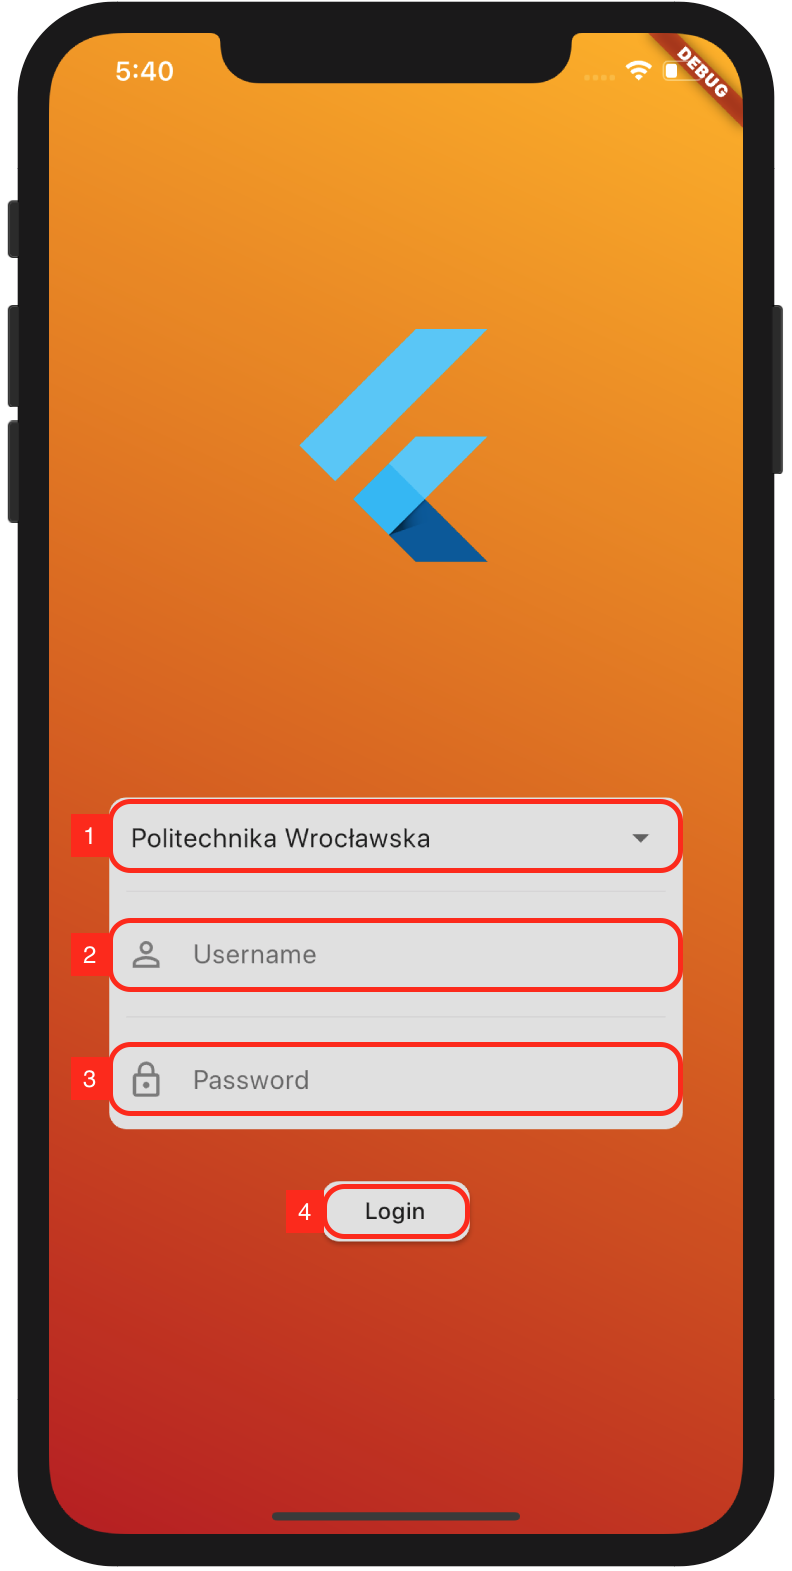
\includegraphics[width=0.3\textwidth]{figC/login_page.png}} &
        {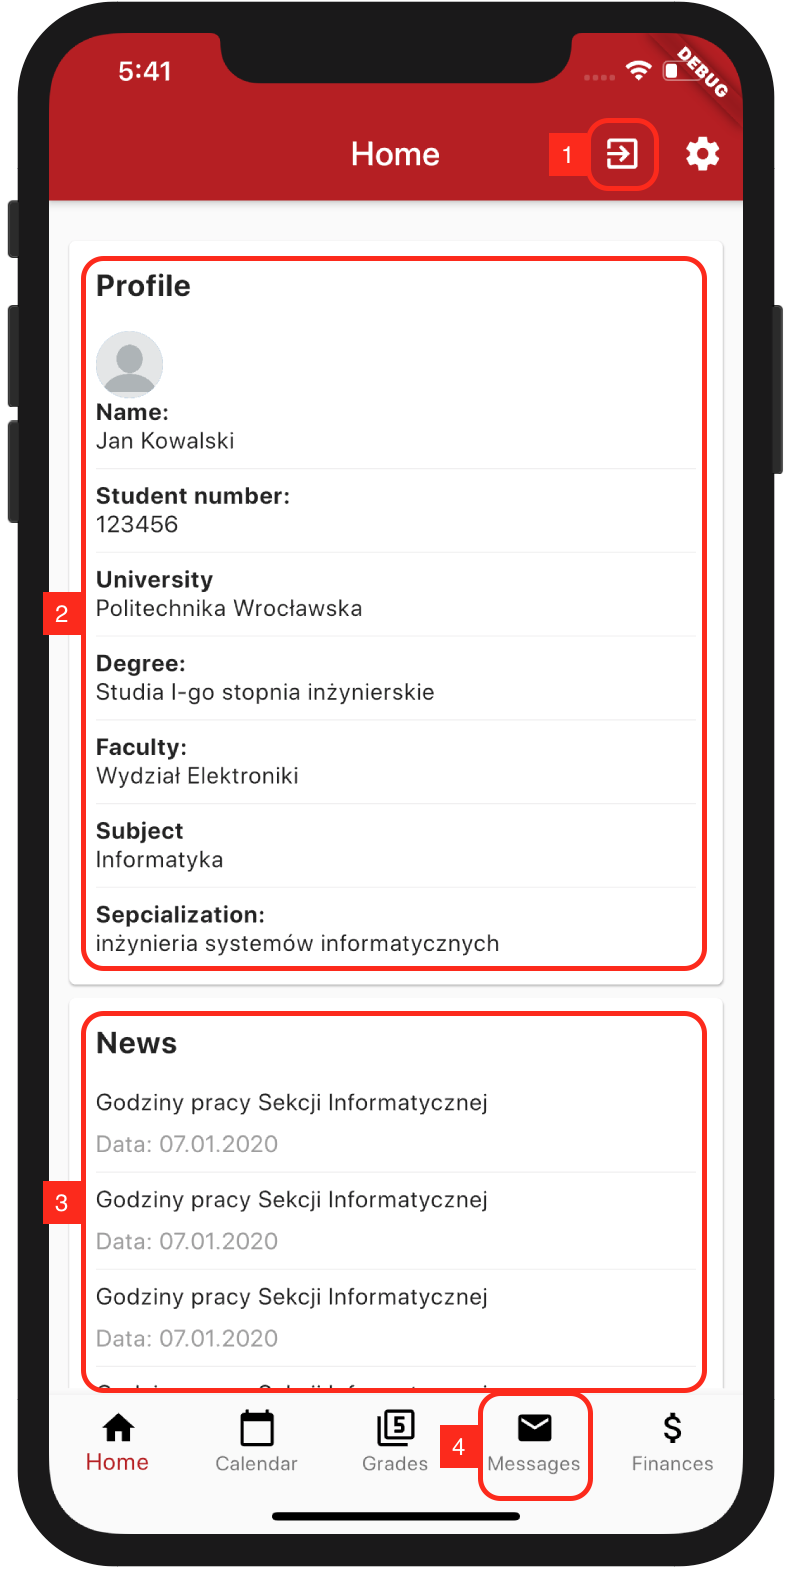
\includegraphics[width=0.3\textwidth]{figC/home_page.png}} \\
    \end{tabular}
    \caption{User's guide: a) login page, b) homepage} \label{fig:users-guide-login-home}
\end{figure}

After the successful login users are redirected to the homepage (Fig.~\ref{fig:users-guide-login-home}b), where they can see sections:
\begin{enumerate}
    \item logout button;
    \item user profile information;
    \item news feed;
    \item link to the messages page.
\end{enumerate}

When users click on the link, they are redirected to the messages page (Fig.~\ref{fig:users-guide-message-and-details}a). Where there are two segments:
\begin{enumerate}
    \item message entries;
    \item navigation with a link to the homepage.
\end{enumerate}

Just after users select one of the messages from the list, they are moved to another screen shown in Figure~\ref{fig:users-guide-message-and-details}b. The message details page is composed of:
\begin{enumerate}
    \item back button - used to get back to the messages page;
    \item message details;
    \item message content.
\end{enumerate}

\begin{figure}[htb]
    \centering
    \begin{tabular}{@{}ll@{}}
        a) & b) \\
        {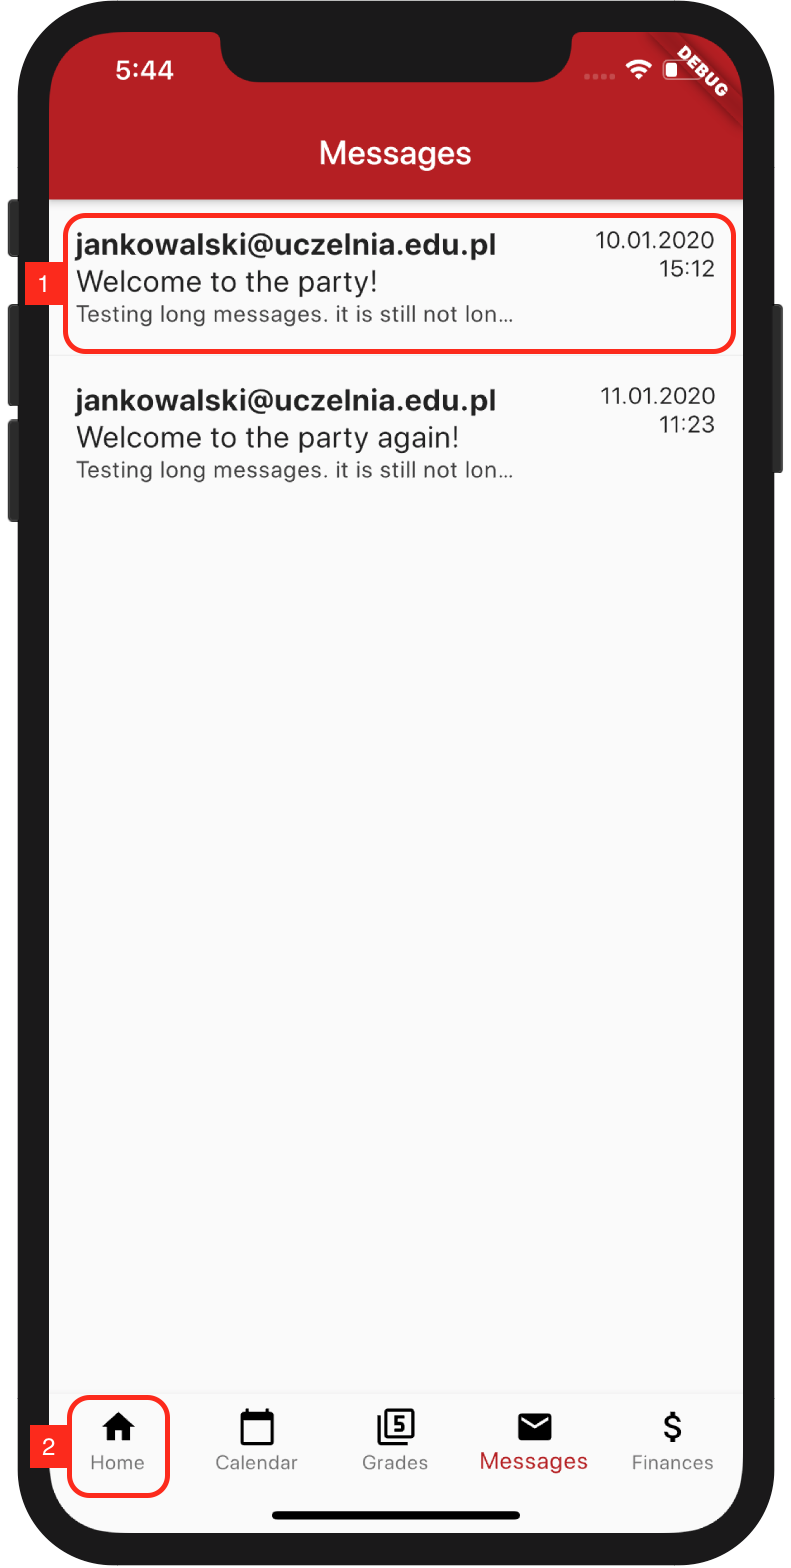
\includegraphics[width=0.3\textwidth]{figC/messages_page.png}} &
        {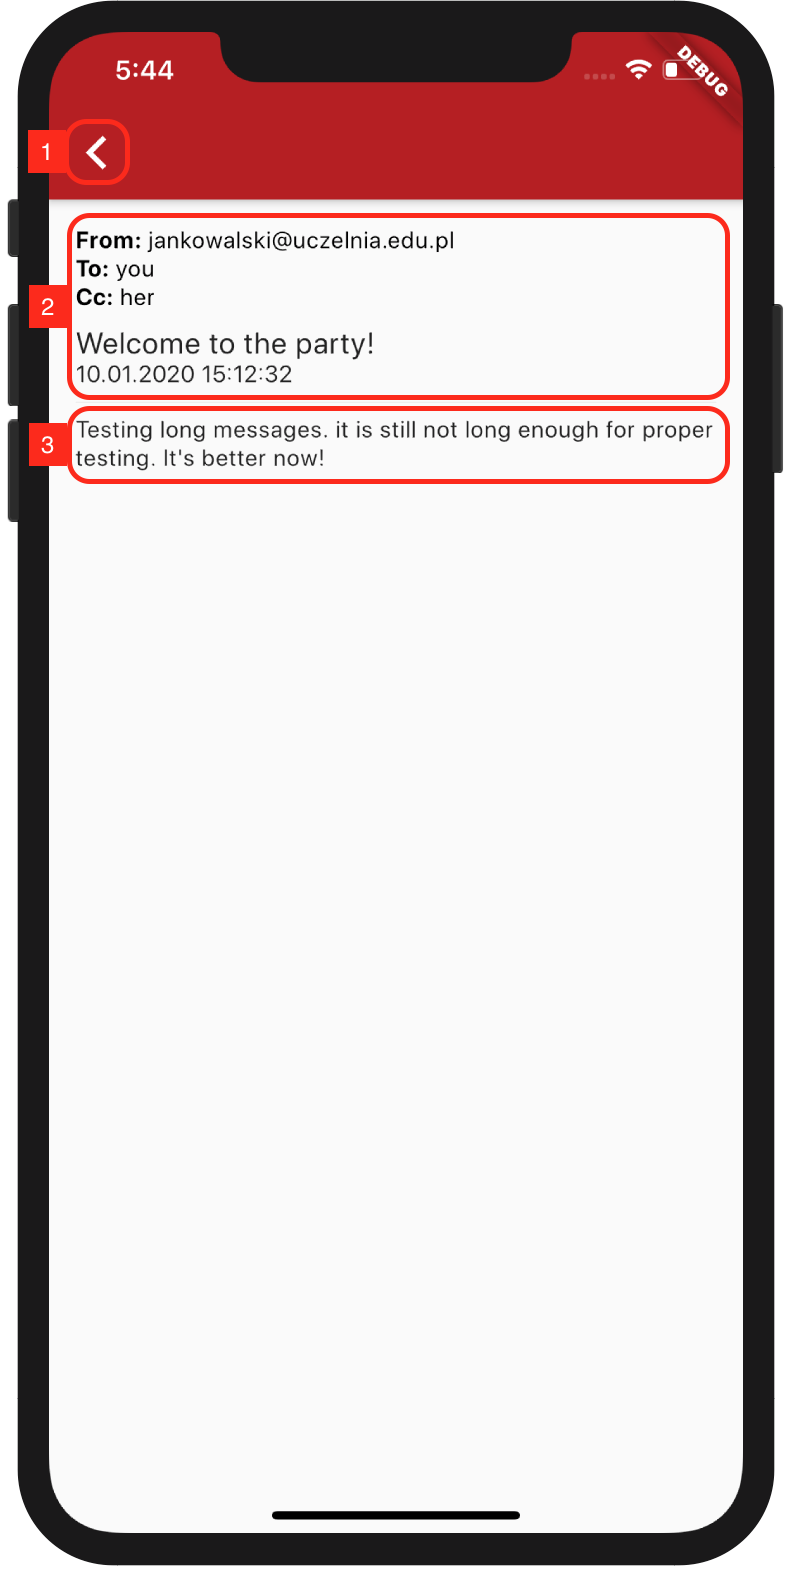
\includegraphics[width=0.3\textwidth]{figC/message_details.png}} \\
    \end{tabular}
    \caption{User's guide: a) messages page, b) message details page} \label{fig:users-guide-message-and-details}
\end{figure}
